\chapter{Case Study}
% \label{ch:relatedwork}
In this case study, we will discuss how energy consumption is affected if we were to use a containerized environment 
rather than running an application natively. We will also briefly discuss how Lingua Franca, a polyglot coordination 
language for distributed programming, may also contribute towards optimizing energy consumption \textemdash 
albeit for only very specific use cases. 
\section{Docker}
As discussed in Section II, Docker \cite{turnbull_2014} is a container framework which has gained massive 
popularity and real-world application in the past few years. From applications to distributions, one can run 
almost anything inside a containerized environment. Figure \ref{fig:dockerfile} displays a sample 
Dockerfile, which is a script to configure the containerized environment. It can be customized as to one's liking 
and is one of the reasons why Docker has such diverse applications. \\

\begin{figure}
    \begin{center}
        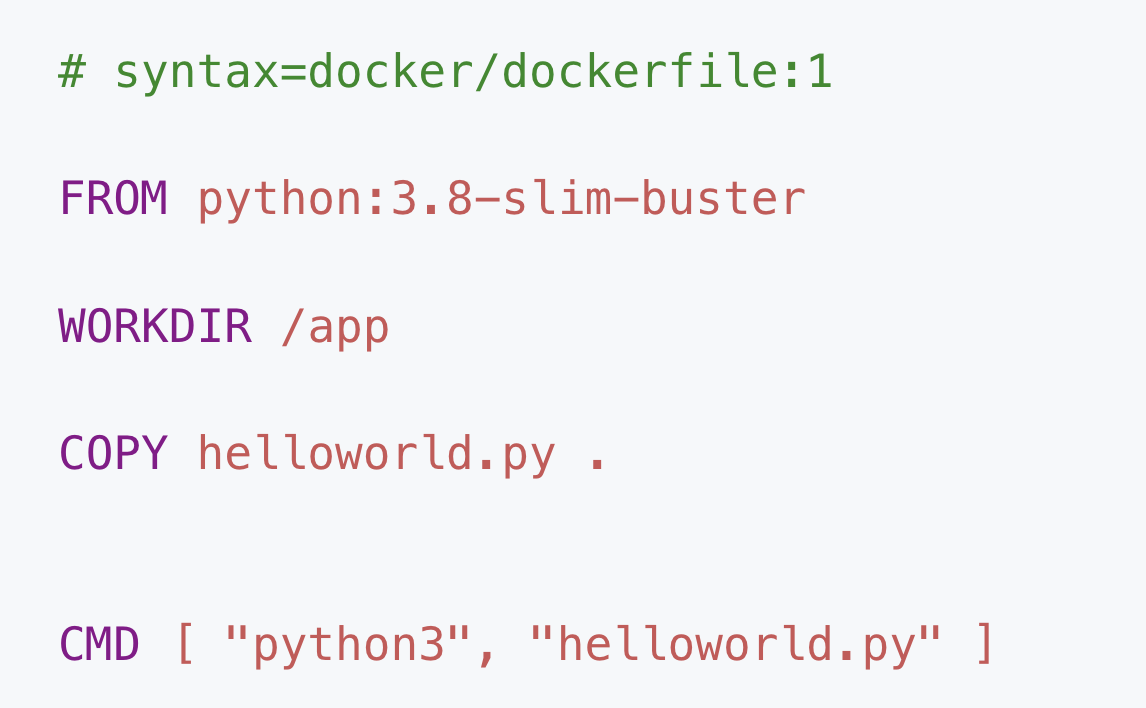
\includegraphics[scale=0.35]{Figs/dockerfile.png}    
    \end{center}
    \caption{A sample Dockerfile}
    \label{fig:dockerfile}
\end{figure}

For this study, we ran \texttt{TempSensClient} as a Docker container on the Raspberry Pi \textemdash we will call 
it \texttt{TempSensClientDocker}. The only thing extra that 
needed to be done was forwarding the port for socket communication when starting up the container. This is due to the 
fact that Docker abstracts the networking layer so the container ports are different from the host ports. The 
assumption for this study was that \texttt{TempSensClientDocker} would consume more energy than \texttt{TempSensClient}. 
However, since we are more interested in communication cost and the energy associated with it, we wanted to 
compare the communication cost. Figure \ref{fig:dockerenergy} shows the EPB for \texttt{TempSensClientDocker} w.r.t 
each chunk size. \\

\begin{figure}
    \begin{center}
        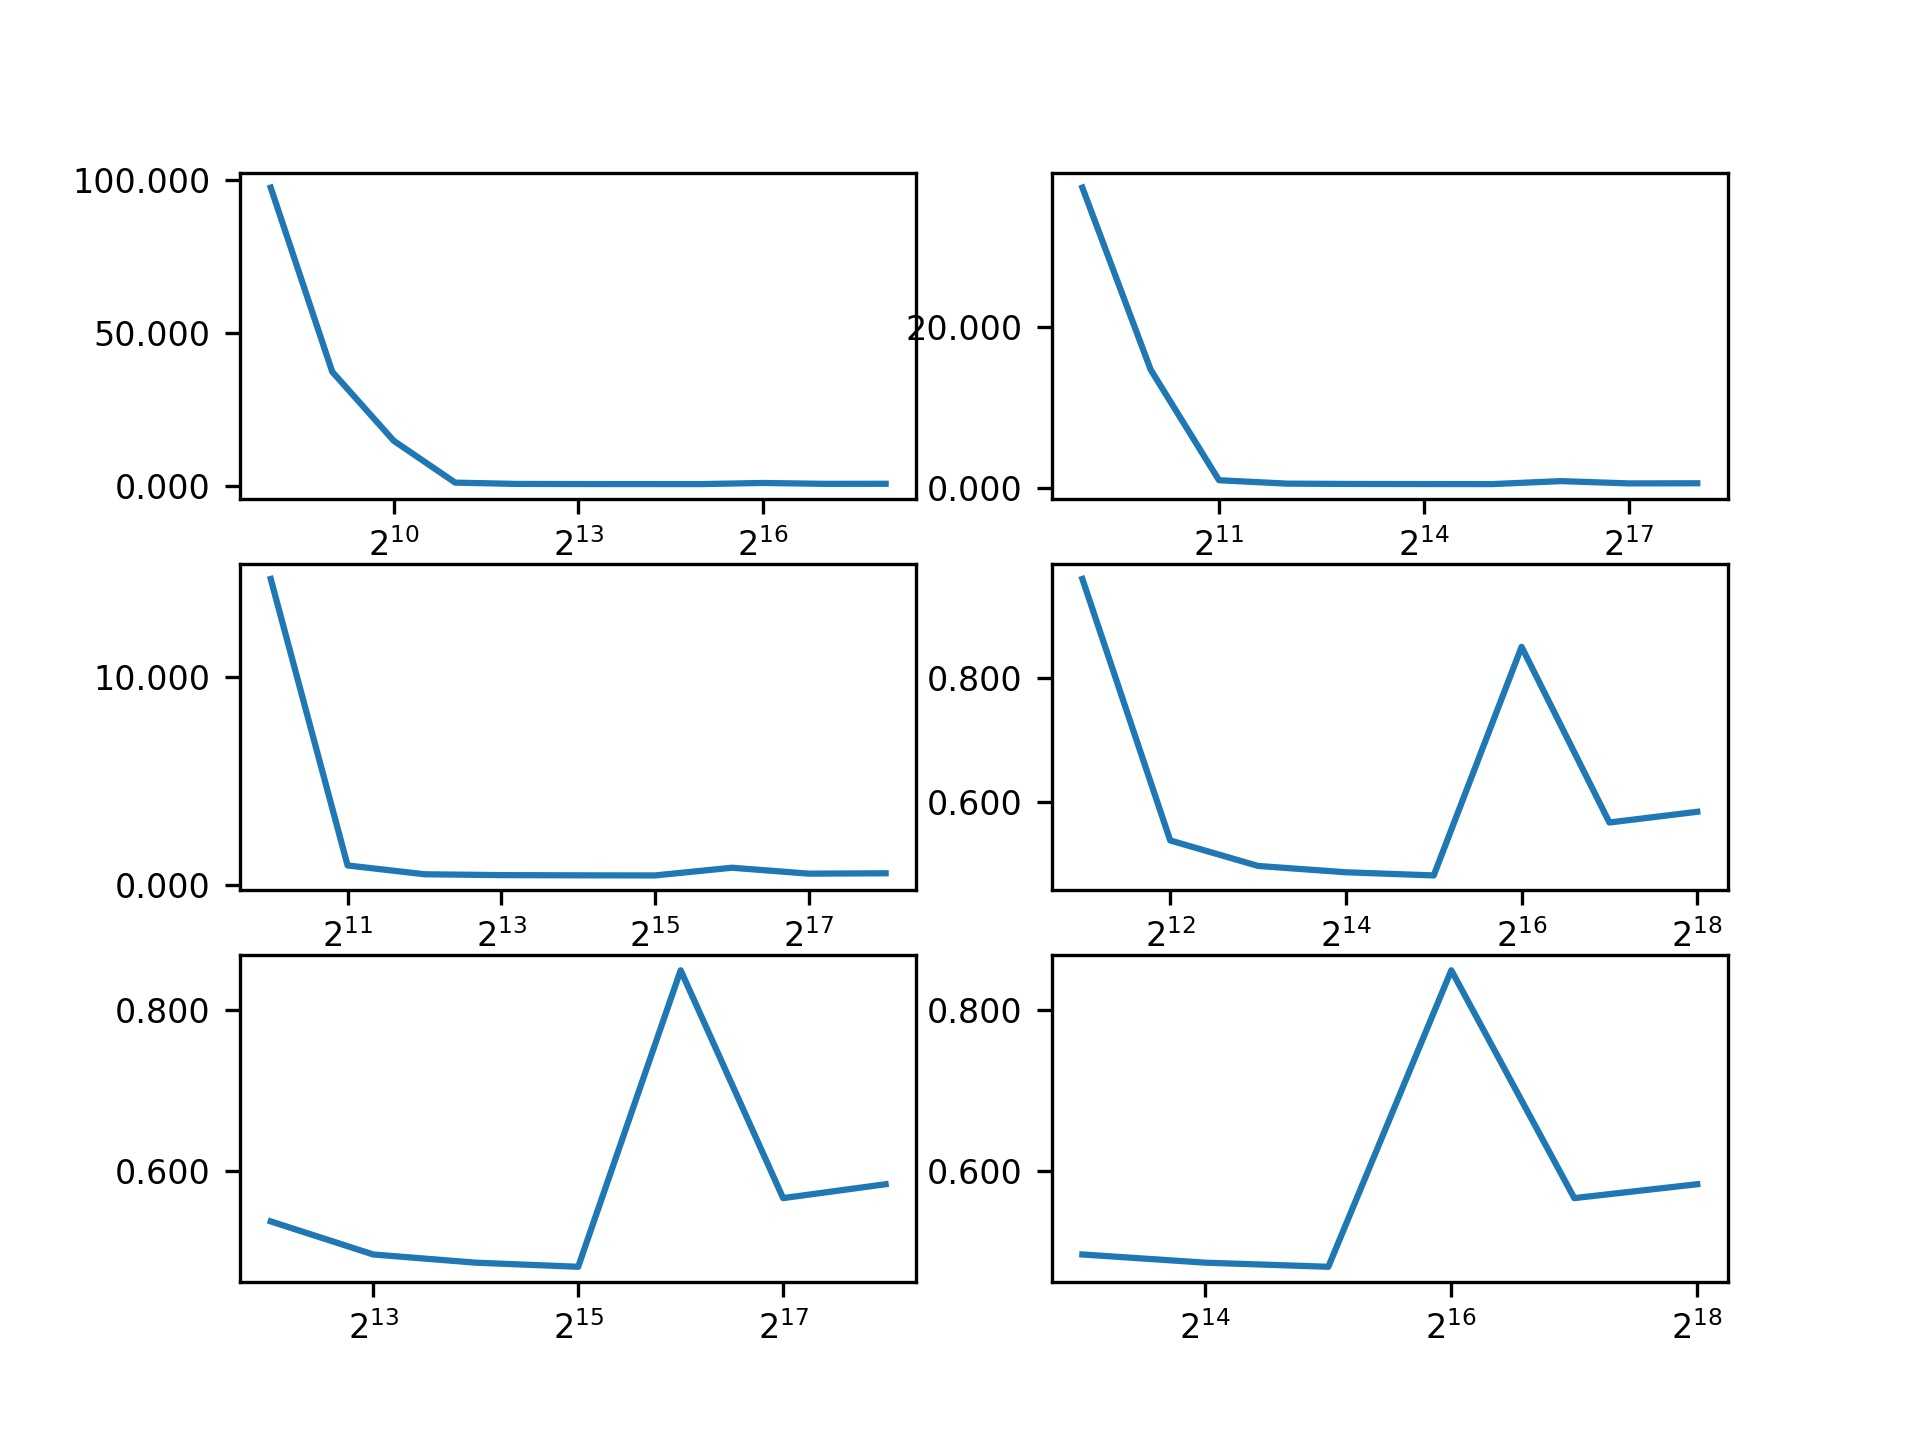
\includegraphics[scale=0.23]{Figs/dockerenergy.png}    
    \end{center}
    \caption{EPB for different chunk sizes (Chunk Size (x-axis) and Energy in microJ (y-axis)) - Raspberry Pi 4 (Docker)}
    \label{fig:dockerenergy}
\end{figure}

This experiment shows that the optimal chunk size for \texttt{TempSensClientDocker} is $2^{15}$ unlike \texttt{TempSensClient} 
that had an optimal chunk size of $2^{14}$. Even though we did expect a little difference between the energy 
consumption, what we did not anticipate was getting a completely different optimal chunk size for the same size on 
the same hardware configuration. Running an application adds an overhead in terms of energy consumption but on the 
other hand provides more maintainability and process isolation. However, the different optimal chunk size is not 
a result of that. As we discussed before, Docker abstracts the networking layer (among other things such as the file 
system) and in order for \texttt{TempSensClientDocker} to be able to communicate with \texttt{TempSensServer} over 
WiFi, we needed to forward the port that the application is supposed to listen at. Recall that in order to compute 
energy consumption, we need both power and time. The power factor here is static and the same as \texttt{TempSensClient} 
however, the abstraction and port forwarding adds to the time factor and therefore, \texttt{TempSensClientDocker} takes 
a tiny bit longer to communicate as compared to \texttt{TempSensClient}, and therefore, has a different optimal chunk size. \\

One question that we would like to ask is that would it be viable to use Docker to achieve energy efficiency? From 
our experiment, it is clear that the optimal chunk size is different and the energy consumption corresponding 
to that is higher than \texttt{TempSensClient} as well. We believe that for the sake of running a single application 
in containerized environment, it is not worth the trade to consume more energy as maintaining one application is 
a somewhat easier task. However, if multiple applications are running inside the same container, then we 
could minimize some of the overhead costs and have a trade-off between maintainability and energy consumption 
depending on the use-case. But, the energy consumption while using Docker would still be greater than running the 
application on a bare-metal OS. This is due to the fact that containers are based on virtualization 
and the I/O system calls that interact with the machine as well as abstractions (such as network layer) 
have a specific overhead. This effect is also discussed by Santos et al. \cite{DBLP:journals/corr/abs-1011-0686} and explains why energy consumption 
is different in a container environment. 

\section{Lingua Franca}
Lingua Franca is a framework developed to provide a coordination language for distributed systems. There are a 
lot of things it is capable of but for the sake of this study, we will focus on features that best relate to 
our work. \\
One of the things that was most interesting was how after writing an LF program, the tool produced efficient code 
for the target programming language. Moreover, it introduces the notion of logical and physical time. Logical time 
is instantiated the moment the program is executed with the system clock's value, which is just the physical time 
at that point. However, logical time progresses differently than physical time. Logical time does not advance 
during the execution of the reaction unlike physical time. Which means that all reactions inside a specific reactor 
are instantaneous. In other terms, two reactions can run concurrently as long as proper variable value handling is done. 
Our assumption was that this could mean the code will execute faster (if possible) given the necessary variables 
had their values instantiated at all possible times, or if the wait time was very minimal. This would further 
help in reduced energy consumption if the program took lesser than usual execution time (with the one time overhead 
of writing the LF equivalent and generating the application code). The code below \cite{lfsource} is an example of concurrent 
reactions being run simultaneously and how the second reaction will print the same result but the process 
 is dependant on 
first reaction's output. To put it simply, if \texttt{out} is set before \texttt{out.is\_present} is called in the 
second reaction, it will double the output and print 42. Otherwise, it will just print 42 (from the \texttt{else} condition) since there is no logical 
information available to determine the wait time in this example. This also show-cases how we can improvise and 
avoid non-determinism. But how much of this actually helps when the application in question is sequential 
and pretty straightforward in question? How does the efficient code generation impact code generation? \\

\begin{lstlisting}{language=Python}
    reactor Source {
    output out;
    preamble {=
        import random
    =}

    reaction(startup) -> out {=
        # Set a seed for random number generation based on the current time.
        self.random.seed()
        # Randomly produce an output or not.
        if self.random.choice([0,1]) == 1:
            out.set(21)
    =}
    reaction(startup) -> out {=
        if out.is_present:
            out.set(2 * out.value)
        else:
            out.set(42)
    =}
    }
\end{lstlisting}

We implemented \texttt{TempSens} purely as an LF application with \texttt{TempSensClientLingua} and 
\texttt{TempSensServerLingua}. The EPB results were similar to Figure \ref{fig:epbpi} because the Python 
source code generated by LF from the above versions was about 99\% identical to our original version. This 
is due to the fact that our application was very simple in nature and also had none of the distributed elements 
that LF could take advantage of. However, we implemented a basic matrix multiplication program in Python 
utilizing parallelism via multi-threading, and then created an LF version for it (see Appendix A). The LF generated 
version was 1.742 seconds slower than the original Python program. There are a number of reasons behind this. 
First, LF has its own overhead because it keeps tracks of logical time among other things. Second, multi-threading 
is not possible using Python since it is not a thread-safe language. The only type of parallelism that can be 
obtained is via multi-processing. And to the best of our knowledge, there is no current LF implementation alternative 
to pool and collect data from multiple processes. \\

The motivation behind this study was to determine whether LF generated programs are more energy-efficient or 
not. From our study, we found out that is not the case with sequential programs with no distributed element 
to them. The \texttt{TempSensClientLingua} took more overall time for communication and hence consumed more energy than 
\texttt{TempSensClient} even though the communication cost was comparable. We believe that since it is designed for 
distributed applications, it would be able to generate more efficient code. However, we also believe that 
the communication cost would not be affected by it since it is not a distributed programming construct but 
since the overall program will be potentially more efficient (due to ease of implementation and understanding 
through LF) in terms of energy consumption. \\
We wanted to conduct a study for the Fall Detection application as well but weren't able to do so due to 
technical limitations. If Fall Detection application were to be implemented as a distributed application, 
we believe that the source code generated by LF would be more energy-efficient. This stems from the fact that 
LF programs are highly specific in terms of functionality without the need for any code bloat, and are 
easier to translate distributed concepts into. This results in less ambiguity and redundancy in the generated 
code and therefore, with fewer instructions to process, it would consume less energy than its natively written 
counterpart. \\
We will discuss the technical limitations in detail in the next section where we will conclude our thesis.